\documentclass[a4paper]{article}
\usepackage{latexsym,amssymb,amsmath,amsbsy,amsopn,amstext,xcolor,multicol}
\usepackage{ctex,hyperref,graphicx,wrapfig,fancybox,listings}
\usepackage{pgf,pgfarrows,pgfnodes,pgfautomata,pgfheaps,pgfshade}
\usepackage[top=1in, bottom=1in, left=1.25in, right=1.25in]{geometry}
\graphicspath{{pic/}}
\title{\bf 电子学基础第二次仿真作业报告}
\date{2017.12.9}
\author{计64~翁家翌~2016011446}
\begin{document}
\kaishu
\ttfamily
\maketitle
%\tableofcontents
%\newpage
\section{通过仿真画出NMOS和PMOS在不同栅压下的$I_D$-$V_{DS}$曲线,并从图中的取值得出$V_{od}$随着$V_{GS}$的变化关系}
\subsection{仿真电路图}
\begin{figure}[htp]
\centering

\includegraphics[width=1.0\linewidth]{01.png}
\caption{左侧为NMOS,右侧为PMOS}
\end{figure}
\subsection{NMOS 的 $I$-$V$ 特性曲线}
\begin{figure}[htp]
\centering
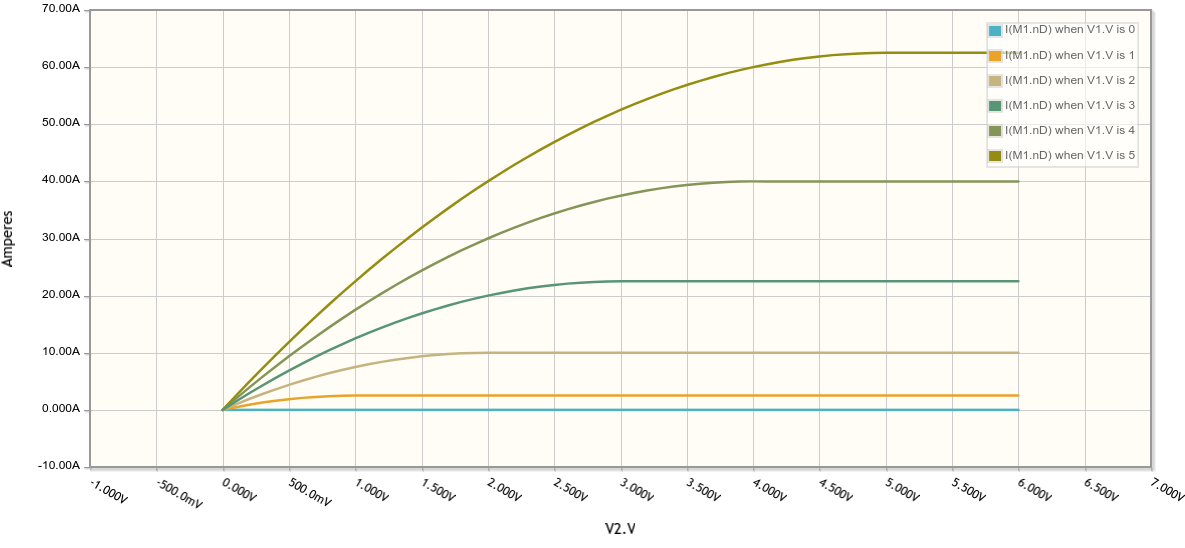
\includegraphics[width=1.0\linewidth]{1.png}
\caption{从下至上依次为$V_1=0,1,2,3,4,5$V}
\label{fig:1}
\end{figure}
\subsection{PMOS 的 $I$-$V$ 特性曲线}
\begin{figure}[htp]
\centering
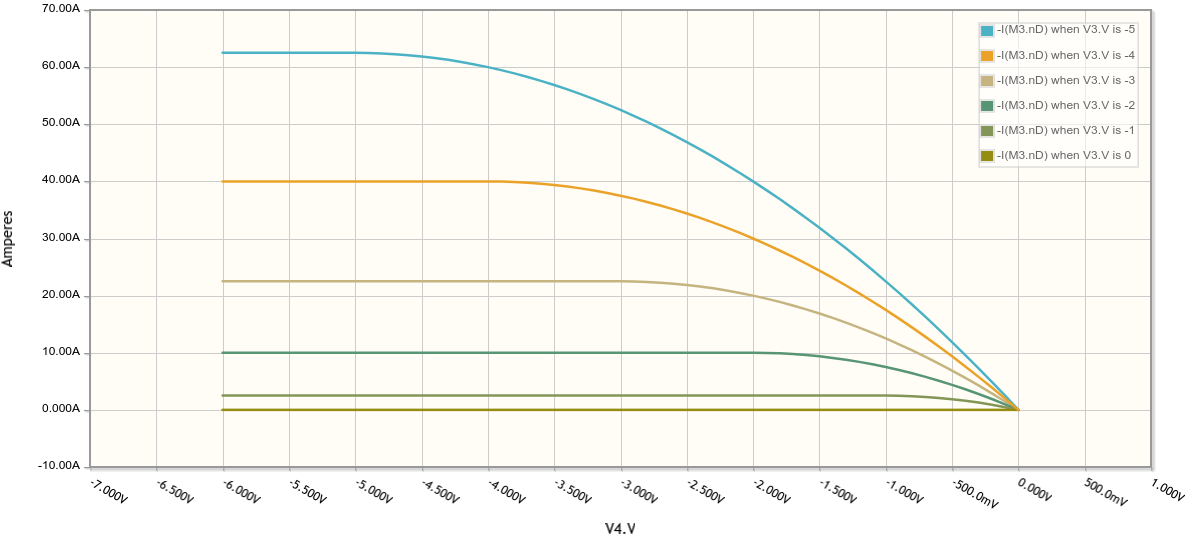
\includegraphics[width=1.0\linewidth]{2.png}
\caption{从下至上依次为$V_3=0,-1,-2,-3,-4,-5$V}
\label{fig:2}
\end{figure}

过驱动电压$|V_{od}|=|V_{GS}|−|V_{th}|$,电路图中所选取的 MOS 管为理想晶体管,故阈值电压 $V_{th}=0$,从图\ref{fig:1}和图\ref{fig:2}的 $I$-$V$ 特性曲线可以看出,在饱和区和线性区的临界点附近,都有$|V_{od}|=|V_{GS}|$,即过驱动电压 $V_{od}$ 随栅源电压 $V_{GS}$ 线性变化。

\section{简单设计两个基本共源放大器,一个是电阻负载,一个是MOSFET负载。并讨论随着输入交流小信号频率的增加,增益的变化。当频率达到何值时,增益比低频时下降3dB?}
\subsection{仿真电路图}
\begin{figure}[htp]
\centering
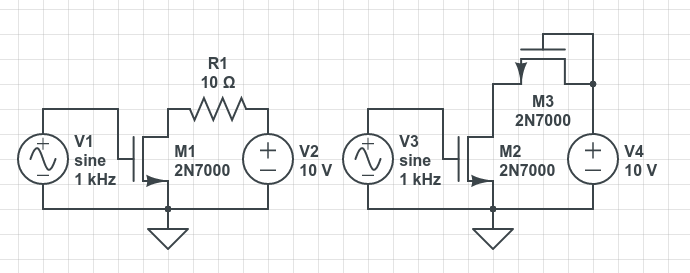
\includegraphics[width=1.0\linewidth]{3.png}
\caption{左侧为电阻负载,右侧为MOSFET负载}
\end{figure}
\subsection{电阻作负载}
交流小信号频率增加超过某个值时,增益开始按一定的斜率降低;如图\ref{fig:3}所示,在低频时$A_v$约为3.01V,即9.57dBV,减弱3dBV后应是6.57dBV,此时的频率约为10.62MHz。
\begin{figure}[htp]
\centering
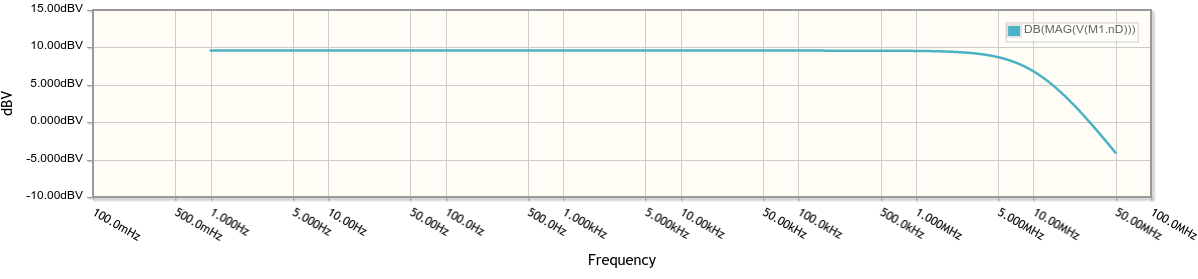
\includegraphics[width=1.0\linewidth]{35.png}
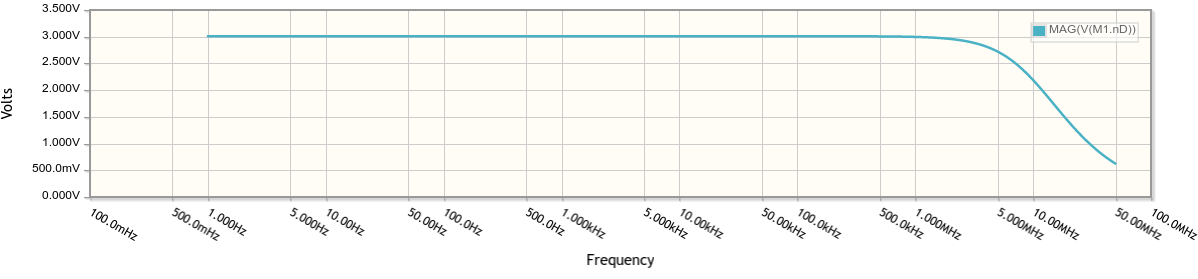
\includegraphics[width=1.0\linewidth]{36.png}
\caption{电阻作负载的共源放大器,上图为dB为单位的$A_v$值,下图为原始$A_v$值}
\label{fig:3}
\end{figure}
\subsection{有源 MOSFET 作负载}
交流小信号频率增加超过某个值时,增益开始按一定的斜率降低;如图\ref{fig:4}所示,在低频时$A_v$约为126.2mV,即-17.98dBV,减弱3dBV后应是-20.98dBV,此时的频率约为27.54MHz。
\begin{figure}[htp]
\centering
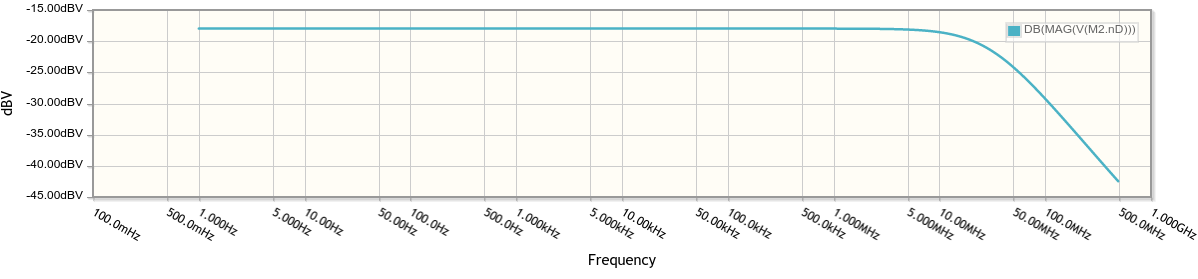
\includegraphics[width=1.0\linewidth]{37.png}
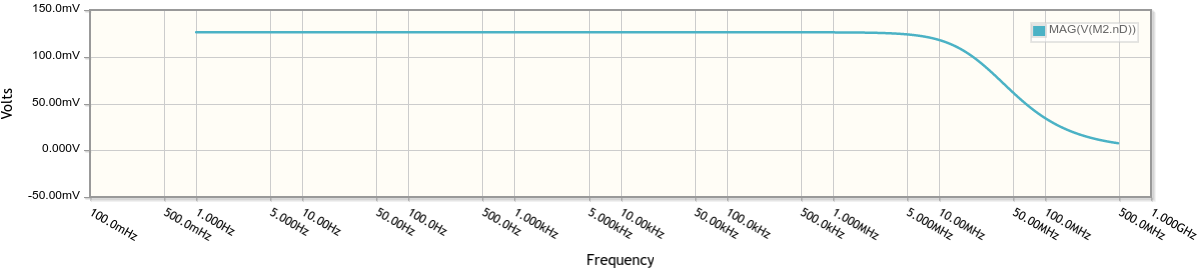
\includegraphics[width=1.0\linewidth]{38.png}
\caption{有源负载共源放大器,上图为dB为单位的$A_v$值,下图为原始$A_v$值}
\label{fig:4}
\end{figure}
\end{document}
